\subchapter{Bootloader - U-Boot}{Objectives: Set up serial
  communication, compile and install the U-Boot bootloader, use basic
  U-Boot commands, set up TFTP communication with the development
  workstation.}

As the bootloader is the first piece of software executed by a
hardware platform, the installation procedure of the bootloader is
very specific to the hardware platform. There are usually two cases:

\begin{itemize}

\item The processor offers nothing to ease the installation of the
  bootloader, in which case the JTAG has to be used to initialize
  flash storage and write the bootloader code to flash. Detailed
  knowledge of the hardware is of course required to perform these
  operations.

\item The processor offers a monitor, implemented in ROM, and through
  which access to the memories is made easier.

\end{itemize}

The Xplained board, which uses the SAMA5D3 SoCs, falls into the second
category. The monitor integrated in the ROM reads the MMC/SD card to
search for a valid bootloader before looking at the internal NAND
flash for a bootloader. In case nothing is available, it will operate
in a fallback mode, that will allow to use an external tool
to reflash some bootloader through USB. Therefore, either by using an MMC/SD
card or that fallback mode, we can start up a SAMA5D3-based board
without having anything installed on it.

\section{Downloading Atmel's flashing tool}

Go to the \code{~/embedded-linux-labs/bootloader} directory.

We're going to use that fallback mode, and its associated tool,
\code{sam-ba}.

We first need to download this tool, from Atmel's website\footnote{
In case this website is down, you can also find this
tool on \url{http://free-electrons.com/labs/tools/}.}.

\begin{verbatim}
wget http://www.atmel.com/Images/sam-ba_2.15.zip
unzip sam-ba_2.15.zip
\end{verbatim}

\section{Setting up serial communication with the board}

Plug the USB-to-serial cable on the Xplained board. The blue end of
the cable is going to \code{GND} on \code{J23}, red on \code{RXD} and
green on \code{TXD}. When plugged in your computer, a serial port
should appear, \code{/dev/ttyUSB0}.

\begin{center}
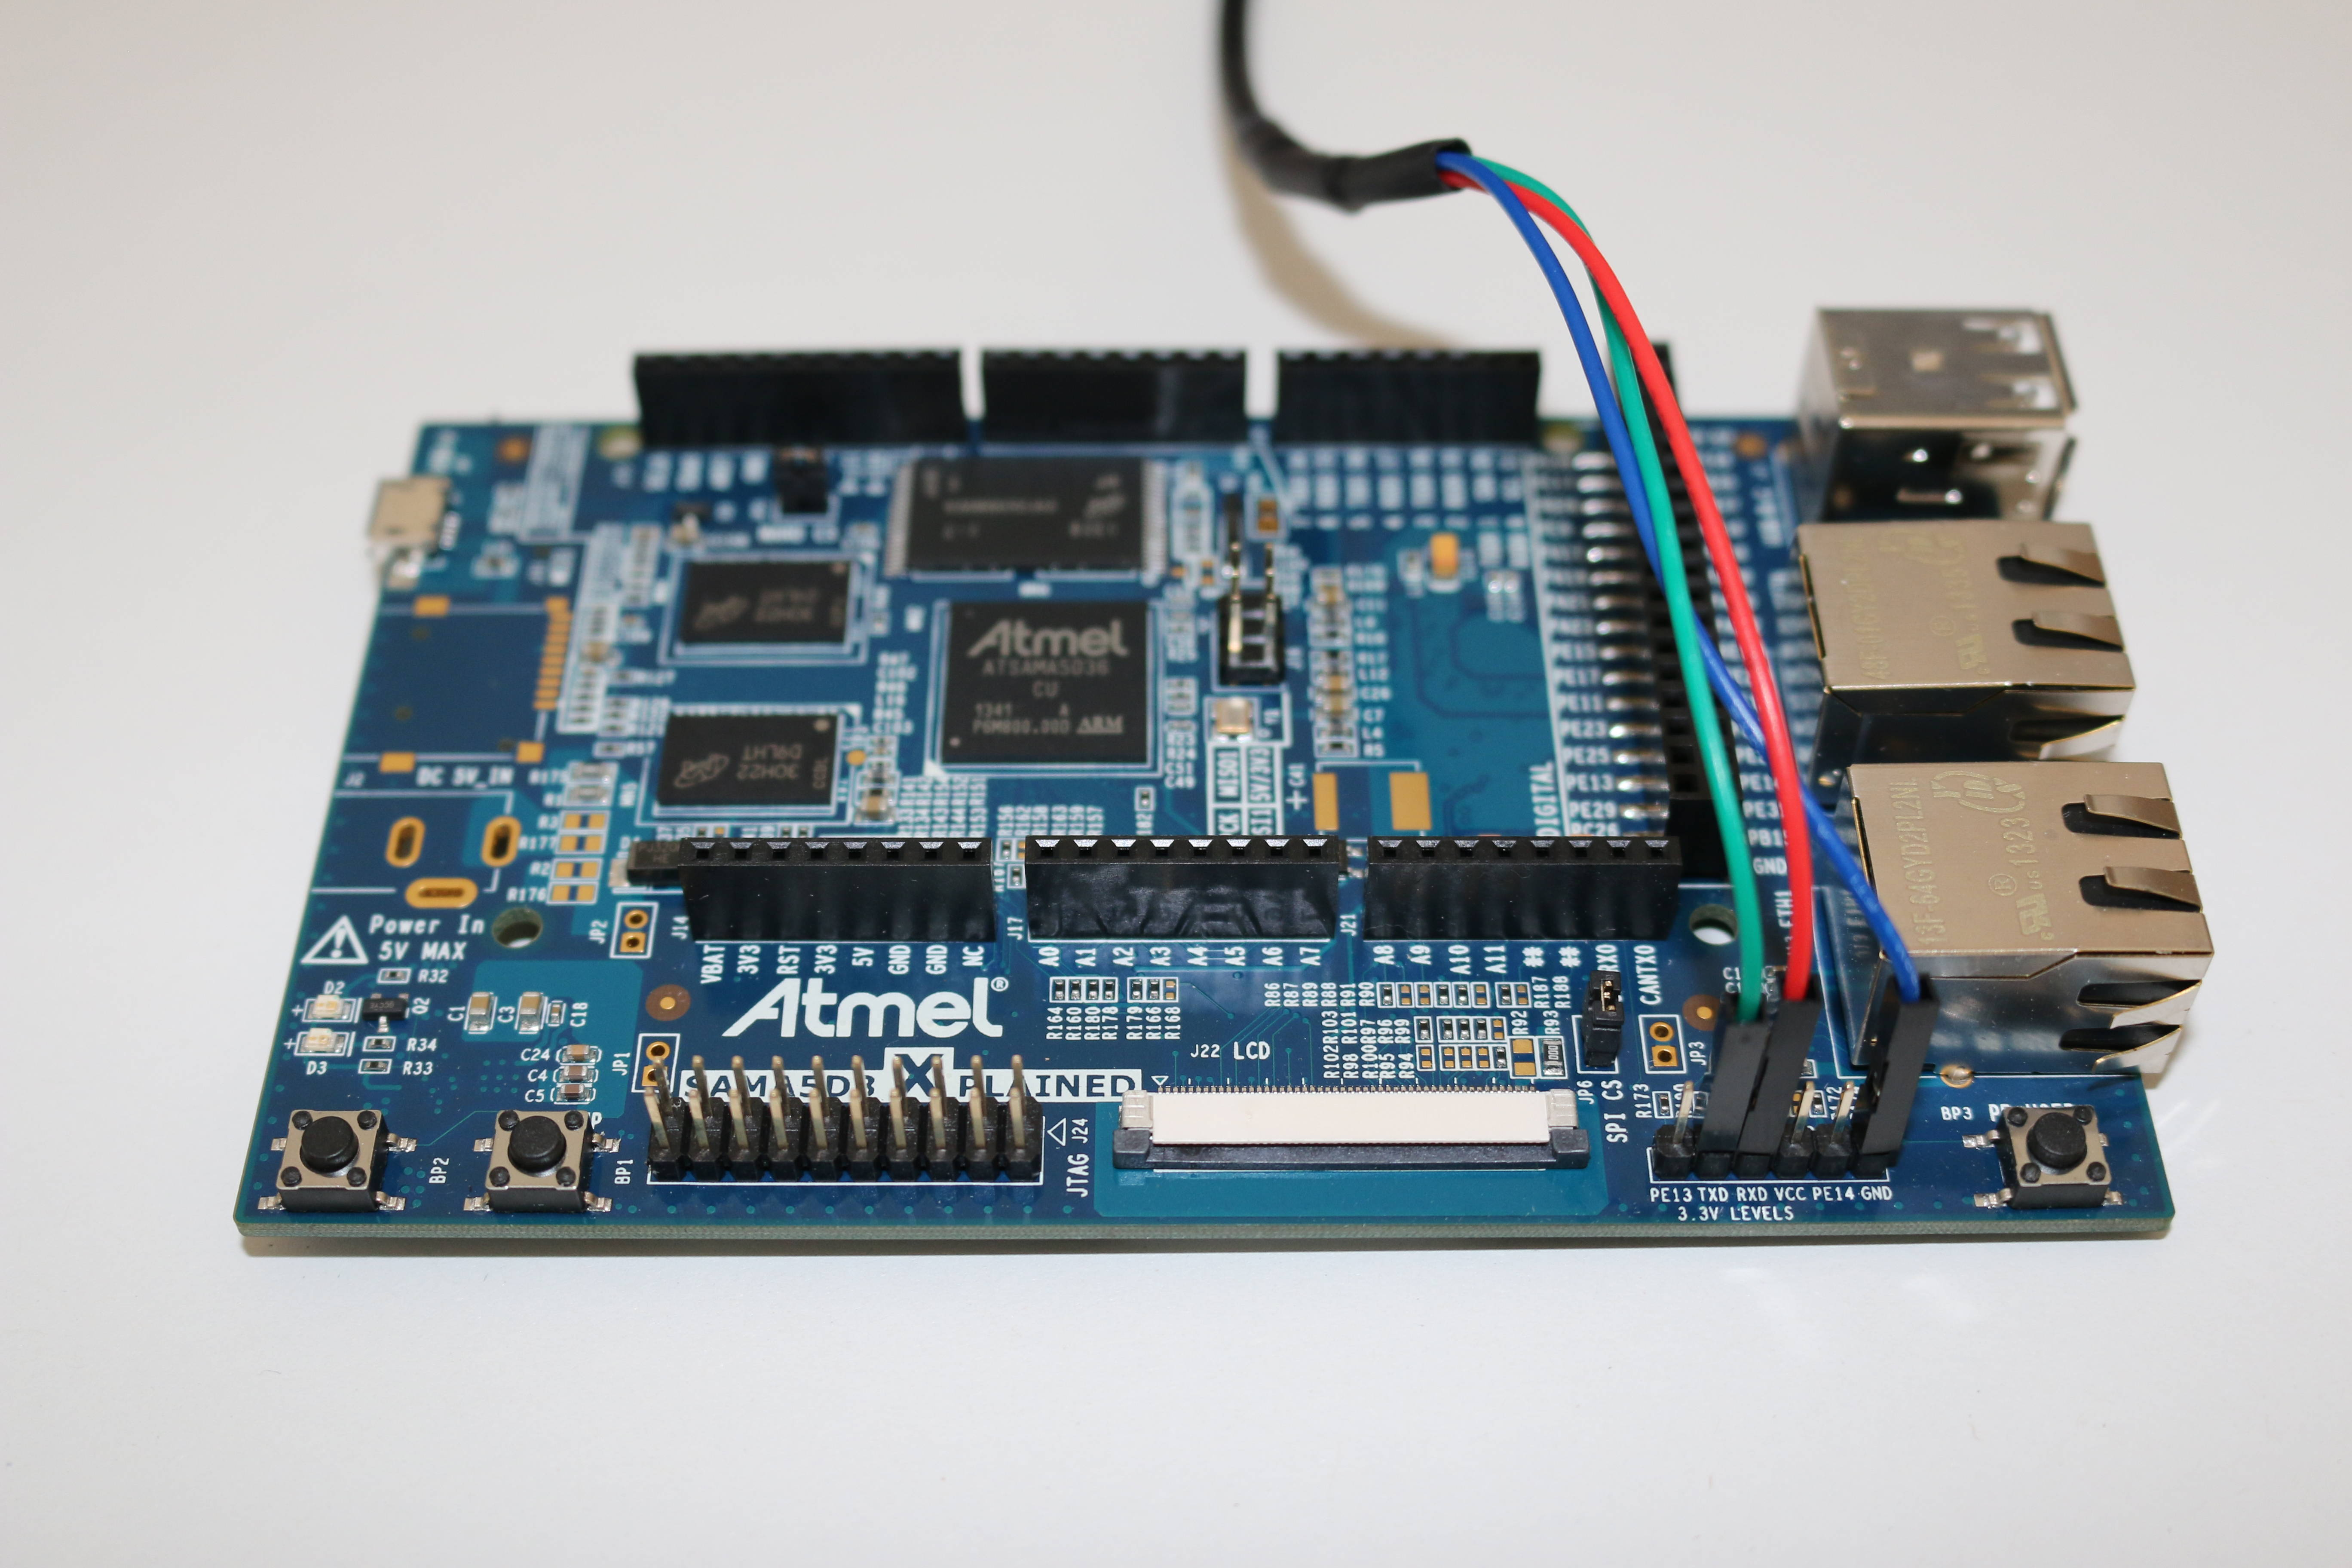
\includegraphics[width=8cm]{labs/sysdev-u-boot/xplained-serial-connector.jpg}
\end{center}

You can also see this device appear by looking at the output of
\code{dmesg}.

To communicate with the board through the serial port, install a
serial communication program, such as \code{picocom}:

\begin{verbatim}
sudo apt-get install picocom
\end{verbatim}

You also need to make your user belong to the \code{dialout} group to be
allowed to write to the serial console:

\begin{verbatim}
sudo adduser $USER dialout
\end{verbatim}

You need to log out and in again for the group change to be effective.

Run \code{picocom -b 115200 /dev/ttyUSB0}, to start serial
communication on \code{/dev/ttyUSB0}, with a baudrate of 115200.

You can now power-up the board by connecting the micro-USB cable to 
the board, and to your PC at the other end. If a system was previously
installed on the board, you should be able to interact with it
through the serial line.

If you wish to exit \code{picocom}, press \code{[Ctrl][a]} followed by
\code{[Ctrl][x]}.

\section{AT91Bootstrap Setup}

The boot process is done in two steps with the ROM monitor trying to
execute a first piece of software, called \code{AT91Bootstrap}, from
its internal SRAM, that will initialize the DRAM, load \code{U-Boot}
that will in turn load Linux and execute it.

As far as bootloaders are concerned, the layout of the NAND flash will
look like:

\begin{center}
  \includegraphics[width=\textwidth]{labs/sysdev-u-boot/flash-map.pdf}
\end{center}

\begin{itemize}
\item Offset \code{0x0} for the first stage bootloader is dictated by
  the hardware: the ROM code of the SAMA5D3 looks for a bootloader at
  offset \code{0x0} in the NAND flash.
\item Offset \code{0x40000} for the second stage bootloader is decided
  by the first stage bootloader. This can be changed by changing the
  AT91Bootstrap configuration.
\item Offset \code{0xc0000} of the U-Boot environment is decided by
  U-Boot. This can be changed by modifying the U-Boot configuration.
\end{itemize}

The first item to compile is AT91Bootstrap that you can fetch from
Atmel's GitHub account:

\begin{verbatim}
git clone git://github.com/linux4sam/at91bootstrap.git
cd at91bootstrap
git checkout v3.7.1
\end{verbatim}

Then, we first need to configure the build system for our setup. We're
going to need a few pieces of information for this:

\begin{itemize}
\item Which board you want to run AT91Bootstrap on
\item Which device should AT91Bootstrap will be stored on
\item What component you want AT91Boostrap to load
\end{itemize}

You can get the list of the supported boards by listing the
\code{board} directory. You'll see that in each of these folders, we
have a bunch of \code{defconfig} files, that are the supported
combinations. In our case, we will load U-Boot, from NAND flash
(\code{nf} in the \code{defconfig} file names).

After finding the right \code{defconfig} file, load it using
\code{make <defconfig_filename>} (just the file name, without
the directory part).

In recent versions of AT91Bootstrap, you can now run \code{make
menuconfig} to explore options available in this program. 

The next thing to do is to specific the cross-compiler prefix
(the part before \code{gcc} in the cross-compiler executable name):

\begin{verbatim}
export CROSS_COMPILE=arm-linux-
\end{verbatim}

You can now start compiling using \code{make}\footnote{You can
speed up the compiling by using the \code{-jX} option with
\code{make}, where X is the number of parallel jobs used for
compiling. Twice the number of CPU cores is a good value.}.

At the end of the compilation, you should have a file called
\code{sama5d3_xplained-nandflashboot-uboot-*.bin}, in the
\code{binaries} folder.

In order to flash it, we need to do a few things. First, remove the
\code{NAND CS} jumper on the board. It's next to the pin header
closest to the Micro-USB plug. Now, press the \code{RESET} button.
On the serial port, you should see \code{RomBoot}.

Put the jumper back.

Then, start \code{sam-ba} (or \code{sam-ba_64} if using a 64 bit
installation of Ubuntu). Run the executable from where it was
extracted. You'll get a small window. Select the \code{ttyACM0}
connection, and the \code{at91sama5d3x-ek} board. Hit \code{Connect}.

You need to:
\begin{itemize}
\item Hit the \code{NANDFlash} tab
\item In the \code{Scripts} choices, select \code{Enable NandFlash}
      and hit \code{Execute}
\item Select \code{Erase All}, and execute the command
\item Then, select and execute \code{Enable OS PMECC parameters}
  in order to change the NAND ECC parameters to what RomBOOT expects.
  Change the number of ECC bits to \code{4}, and the ECC offset to
  \code{36}.
\item Finally, send the image we just compiled using the command
  \code{Send Boot File}
\end{itemize}

AT91Bootstrap should be flashed now, keep \code{sam-ba} open, and move to
the next section.

\section{U-Boot setup}

Download U-Boot:

\begin{verbatim}
wget ftp://ftp.denx.de/pub/u-boot/u-boot-2016.03.tar.bz2
\end{verbatim}


More recent versions may also work, but we have not tested them.

Extract the source archive and get an understanding of U-Boot's
configuration and compilation steps by reading the \code{README} file,
and specifically the {\em Building the Software} section.

Basically, you need to:

\begin{itemize}

\item Set the \code{CROSS_COMPILE} environment variable;

\item Run the \code{tools/genboardscfg.py} utility to generate
      the \code{boards.cfg} file needed in the next step.
\item Run \code{make <NAME>_defconfig}, where \code{<NAME>} is the
  name of your board as declared in \code{boards.cfg}. There are
  two flavors of the Xplained configuration: one to run from the SD card
  (\code{sama5d3_xplained_mmc}) and one to run from the NAND flash
  (\code{sama5d3_xplained_nandflash}). Since we're going to boot on
  the NAND, use the latter. Note that for our platform, both these
  choices are sharing most of their configuration, that is defined in
  \code{include/configs/sama5d3_xplained.h}. Read this file to get an
  idea of how a U-Boot configuration file is written;

\item Now that you have a valid initial configuration, you can now
  run \code{make menuconfig} to further edit your bootloader features. 

\item Finally, run \code{make}, which should build U-Boot.

\end{itemize}

Now, in \code{sam-ba}, in the \code{Send File Name} field, set the path to
the \code{u-boot.bin} that was just compiled, and set the address to
\code{0x40000}. Click on the \code{Send File} button.

You can now exit \code{sam-ba}.

\section{Testing U-Boot}

Reset the board and check that it boots your new bootloaders. You can
verify this by checking the build dates:

\begin{verbatim}
AT91Bootstrap 3.7.1 (Tue May 10 08:59:24 EDT 2016)

NAND: ONFI flash detected
NAND: Manufacturer ID: 0x2c Chip ID: 0x32
NAND: Disable On-Die ECC
NAND: Initialize PMECC params, cap: 0x4, sector: 0x200
NAND: Image: Copy 0x80000 bytes from 0x40000 to 0x26f00000
NAND: Done to load image


U-Boot 2016.03 (May 10 2016 - 09:12:47 -0400)

CPU: SAMA5D36
Crystal frequency:       12 MHz
CPU clock        :      528 MHz
Master clock     :      132 MHz
DRAM:  256 MiB
NAND:  256 MiB
MMC:   mci: 0
*** Warning - bad CRC, using default environment

In:    serial
Out:   serial
Err:   serial
Net:   gmac0
Error: gmac0 address not set.
, macb0
Error: macb0 address not set.

Hit any key to stop autoboot:  0
\end{verbatim}

Interrupt the countdown to enter the U-Boot shell:
\begin{verbatim}
=>
\end{verbatim}

In U-Boot, type the \code{help} command, and explore the few commands
available.

\section{Setting up Ethernet communication}

Later on, we will transfer files from the development workstation to
the board using the TFTP protocol, which works on top of an Ethernet
connection.

To start with, install and configure a TFTP server on your development
workstation, as detailed in the bootloader slides.

With a network cable, connect the Ethernet port labelled ETH0/GETH of
your board to the one of your computer. If your computer already has a
wired connection to the network, your instructor will provide you with
a USB Ethernet adapter. A new network interface, probably \code{eth1}
or \code{eth2}, should appear on your Linux system.

To configure this network interface on the workstation side, click on
the {\em Network Manager} tasklet on your desktop, and select {\em
  Edit Connections}.

\begin{center}
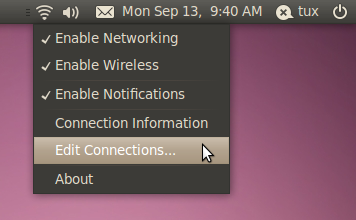
\includegraphics[width=8cm]{labs/sysdev-u-boot/network-config-1.png}
\end{center}

Select {\em Wired connection 1} and press the {\em Edit} button.

\begin{center}
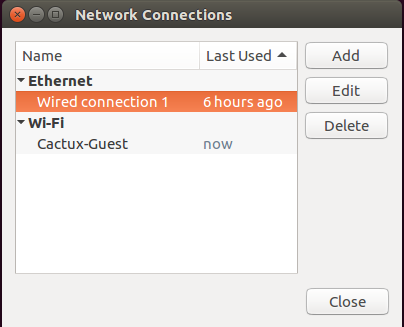
\includegraphics[width=8cm]{labs/sysdev-u-boot/network-config-2.png}
\end{center}

In the \code{IPv4 Settings} tab, choose the \code{Manual} method
to make the interface use a static IP address, like \code{192.168.0.1}
(of course, make sure that this address belongs to a separate network
segment from the one of the main company network).

\begin{center}
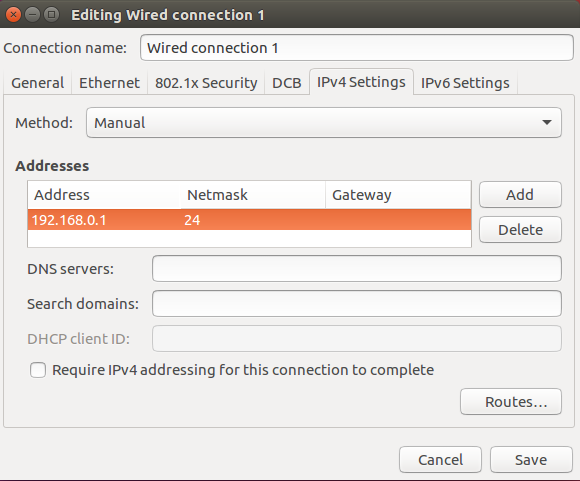
\includegraphics[width=8cm]{labs/sysdev-u-boot/network-config-3.png}
\end{center}

You can use \code{24} as \code{Netmask}, and leave the
\code{Gateway} field untouched (if you click on the \code{Gateway} box, you
will have to type a valid IP address, otherwise you won't be allowed to
click on the \code{Save} button).

Now, configure the network on the board in U-Boot by setting the \code{ipaddr}
and \code{serverip} environment variables:

\begin{verbatim}
setenv ipaddr 192.168.0.100
setenv serverip 192.168.0.1
\end{verbatim}

The first time you use your board, you also need to set the MAC
address in U-boot:

\begin{verbatim}
setenv ethaddr 12:34:56:ab:cd:ef
\end{verbatim}

In case the board was previously configured in a different way, we
also turn off automatic booting after commands that can be used to
copy a kernel to RAM:

\begin{verbatim}
setenv autostart no
\end{verbatim}

To make these settings permanent, save the environment:

\begin{verbatim}
saveenv
\end{verbatim}

Now reset your board\footnote{Resetting your board is needed to
make your \code{ethaddr} permanent, for obscure reasons. If you
don't, U-boot will complain that \code{ethaddr} is not
set.}.

You can then test the TFTP connection. First, put a small text file in
the directory exported through TFTP on your development
workstation. Then, from U-Boot, do:

\begin{verbatim}
tftp 0x22000000 textfile.txt
\end{verbatim}

\fbox{
\begin{minipage}{\textwidth}
{\bf Caution: known issue in Ubuntu 12.04 and later (still present
in Ubuntu 14.04)}: if download through tftp doesn't work,
you may have to stop the \code{tftpd-hpa} server and start it
again every time you boot your workstation:

\code{
sudo service tftpd-hpa restart
}

The problem is Ubuntu starts this server too early, before the
preconditions it needs are met. When you restart the service
long after the machine has booted, this issue is no longer
present.

If it still doesn't work, another (radical!) workaround is to
reinstall the \code{tftpd-hpa} server!

\code{
sudo apt-get install --reinstall tftpd-hpa
}

So far, we haven't had the time yet to investigate the root
cause of the issue that is addressed by this last workaround.
\end{minipage}
}


The \code{tftp} command should have downloaded the
\code{textfile.txt} file from your development workstation into
the board's memory at location \code{0x22000000}\footnote{
This location is part of the board DRAM. If you want
to check where this value comes from, you can check the Atmel SAMA5D3
datasheet at \url{http://www.atmel.com/tools/ATSAMA5D3-XPLD.aspx}, 
following the {\em Documents} link. It's a big document (more than 1,800
pages). In this document, look for \code{Memory Mapping} and you
will find the SoC memory map. You will see that the address range for
the memory controller ({\em DDRC S}) starts at \code{0x20000000}
and ends at \code{0x3fffffff}. This shows that the \code{0x22000000} 
address is within the address range for RAM. You can also try with other
values in the same address range, knowing that our board only has 256 MB
of RAM (that's \code{0x10000000}, so the physical RAM probably ends at
\code{0x30000000}).}.

You can verify that the download was successful by dumping the
contents of the memory:

\begin{verbatim}
md 0x22000000
\end{verbatim}

We will see in the next labs how to use U-Boot to download, flash and
boot a kernel.

\section{Rescue binaries}

If you have trouble generating binaries that work properly, or later
make a mistake that causes you to loose your bootloader binaries, you
will find working versions under \code{data/} in the current lab
directory.
